% Xiangchong
\subsection{Shear estimation}
\subsubsection{Re-Gaussianization}
Galaxy shapes are estimated with the $\galsim$ implementation  of the
re-Gaussianization PSF correction method \citep{Regaussianization}.  The
outputs are two components of the ellipticity:
\begin{equation}
    (e_1,e_2)=\frac{1-(b/a)^2}{1+(b/a)^2} (\cos 2\phi,\sin 2\phi),
\end{equation}
where $b/a$ is the axis ratio, and $\phi$ is the position angle of the major
axis with respect to the equatorial coordinate system.  The resolution factor
$R_2$, which is defined with the trace of the moment matrix of the PSF $T_P$
and that of the observed galaxy image $T_I$ as
\begin{equation}
    R_2=1-\frac{T_P}{T_I},
\end{equation}
is used to quantify how well-resolved the galaxy is compared to the PSF.

For a galaxy ensemble distorted by a constant shear, the shear is estimated
with weighted average ellipticity of galaxies in the ensemble:
\begin{equation}
    (\hat{g_1},\hat{g_2}) = \frac{1}{2\res}\left\langle (e_1,e_2) \right\rangle,
\end{equation}
where the `shear responsivity' $\res$ is the response of the ellipticity to a
small shear.
The ensemble average is weighted with $w_i$, which is defined as
\begin{equation}
    w_i=\frac{1}{\sigma_e^2+e_{\rm{rms}}^2},
\end{equation}
where $e_{\rm{rms}}$ is the root-mean-square ($\texttt{RMS}$) of intrinsic
ellipticity per component. The estimation of $e_{\rm{RMS}}$ and $\sigma_e$
using image simulation is shown in section \ref{subsec:optimal}.
The responsivity for the source population is estimated as
\begin{equation}
    \res=1-\frac{\sum_i w_i e^2_{\rm{rms},i}}{\sum_i w_i}.
\end{equation}

\subsubsection{Bias modeling}


\subsection{Simulation}
\label{subsec:Sim}

\subsubsection{Noise and PSF}

Our simulation is divided into $2500$ sub-samples and each sub-sample contains
$10^4$ postage-stamps with $64\times 64$ pixels. The pixel size is set to
$0.168$ arcesc. The noise property and PSF are the same for galaxies in one
sub-sample while they vary among different sub-samples. The HSC pipeline
reconstruct the PSF models and noise variances at any position of the coadd
images. We collect $2500$ noise variances and PSF models from a set of random
positions on the coadd images of HSC-WIDE layer within the footprint of the HSC
shape catalog.

Noise on the coadd images has spacial correlation due to the warping kernel
used to resample single exposures on the common pixel frame in the coadding
process. We sample the noise correlations from the blank pixels on the coadd
images. The sampled noise correlations, which are noisy at individual level,
are subsequently divided into eight groups and stacked in each group to create
eight different noise correlations with high signal to noise ratio.

Each sub-sample is assigned with a noise PSF model, noise variance and noise
correlation function. We then reweight each subsample to match the seeing
histograms and noise variance histograms of the simulation to the observation.
To note, the HSC WIDE layer is divided six observational fields (XMM, GAMA09H,
WIDE12H, GAMA15H, VVDS, HECTOMAP) and the reweighting is conducted for each
field. The seeing histograms and noise variance histograms of the observation
and simulation are shown in Figure \ref{fig:noiHist} and Figure
\ref{fig:fwhmHist}.

\begin{figure*}[ht!]
\centering{
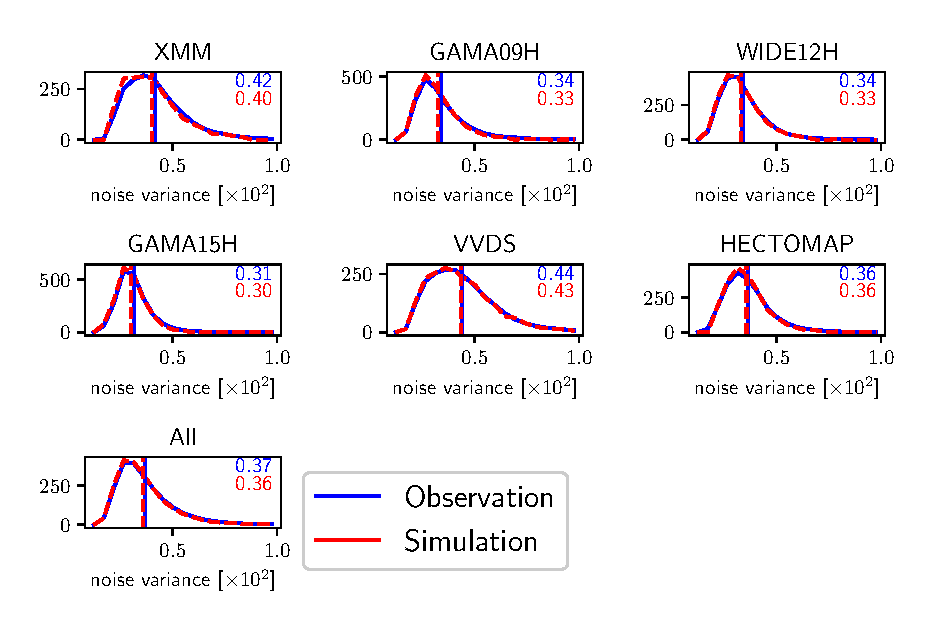
\includegraphics[width=0.9\textwidth]{noiVar_reCheck_recut.eps}
}
\caption{The first $6$ panels show the number histograms of noise variance for
    $6$ fields of the observation and the simulation. The last panel shows the
    histograms for the galaxies in all of the fields. The blue solid lines
    denote the observation and the red dashed lines denote the simulation. The
    blue texts show the average noise variance of the observation while the red
    texts show the average noise variance of the simulation.
    }
\label{fig:noiHist}
\end{figure*}

\begin{figure*}[ht!]
\centering{
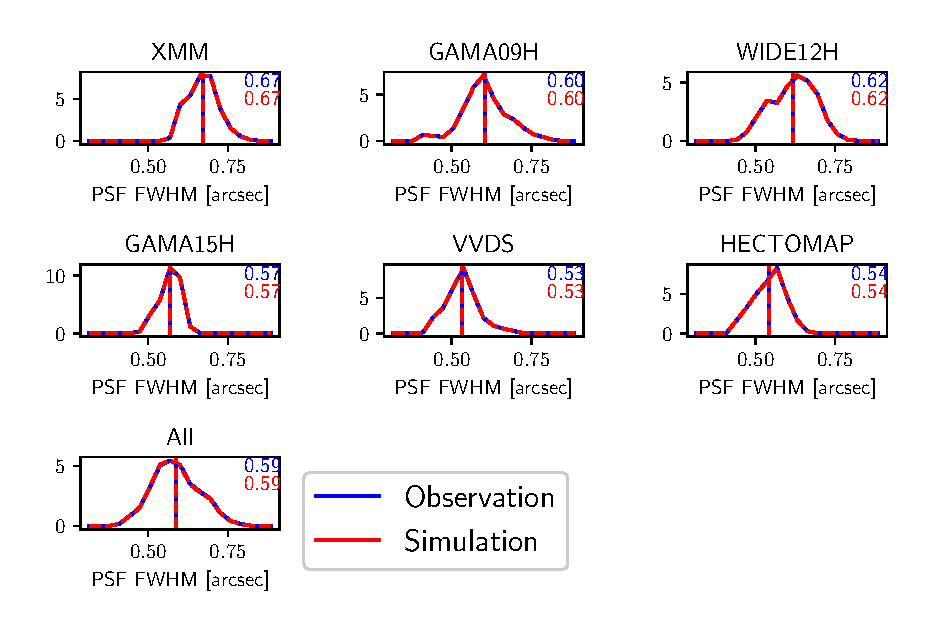
\includegraphics[width=0.9\textwidth]{psfFWHM_reCheck_recut.eps}
}
\caption{The first $6$ panels show the number histograms of noise variance for
    the $6$ fields of the observation and the simulation. The last panel shows
    the histograms for the galaxies in all of the fields. The blue solid lines
    denote the observation and the red dashed lines denote the simulation. The
    blue texts show the average FWHM of the observation while the red texts
    show the average FWHM of the simulation.
    }
\label{fig:fwhmHist}
\end{figure*}

\subsubsection{Galaxies}
We use the galaxy training sample created by \citet{HSC1-GREAT3Sim} as our
input galaxies. \citet{HSC1-GREAT3Sim} selects galaxies from the HSC WIDE-DEPTH
coadds \citep{HSC1-data} with CModel magnitude less than $25.2$.  Subsequently,
\citet{HSC1-GREAT3Sim} finds the centers of these selected galaxies on the
COSMOS-HST \citep{HST-ACSpipe} exposures and cuts out postage-stamps around
these positions. These positions are set to as the centers of the
postage-stamps and the postage sizes are required to be larger than $10.75$
arcsec to contain the galaxy light and structures of neighboring sources.

\citet{HSC1-GREAT3Sim} creates three training samples from three WIDE-DEPTH
coadds with different seeing values which are 0.5\arcsec, 0.7\arcsec and
1.0\arcsec. We use the training sample with the best seeing as our input galaxy
sample since it has the largest number of galaxies.

$\galsim$ \citep{Galsim}, which is an open-source package for galaxy image
simulation, is used to simulate the HSC-like postage-stamps from the COSMOS HST
postage-stamp. The PSF is deconvolved from each input postage-stamp and then
the postage-stamp is convolved with an assigned HSC PSF model. The original
noise is whitened for each postage stamp then a noise with an assigned HSC
variance and HSC nosie correlation function is added to the postage-stamp.

\subsubsection{Image Processing} HSC pipeline is being developed to process the
data of HSC survey and will finally be applied to LSST survey. We use HSC
pipeline to detect galaxies from the simulated images and isolate blended
galaxies with HSC deblender to define a sample of sources. Subsequently, the
HSC pipeline is used to perform magnitude and shape measurements on the
detected sources.

\begin{figure*}[ht!]
\centering{
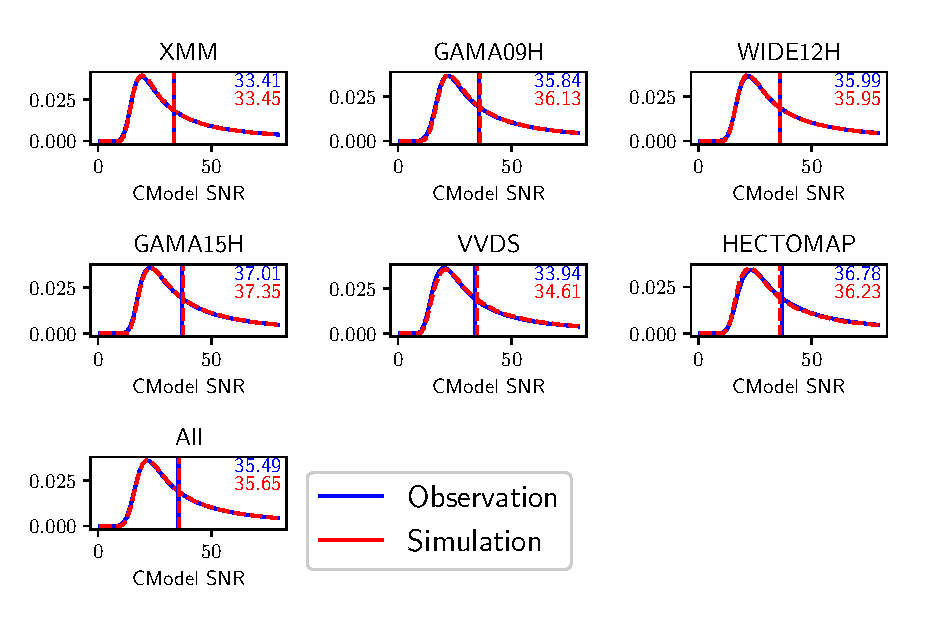
\includegraphics[width=0.9\textwidth]{snrDis_reCheck.eps}
}
\caption{The first 6 panels compare the number histograms of CModel SNR between
    the observation and the simulation for galaxies in 6 fields of the second
    year HSC shape catalog. The last panel shows the histograms for the
    galaxies in all of the fields. The blue solid lines are for the observation
    and the red dashed lines are for the simulation.
    }
\end{figure*}

\begin{figure*}[ht!]
\centering{
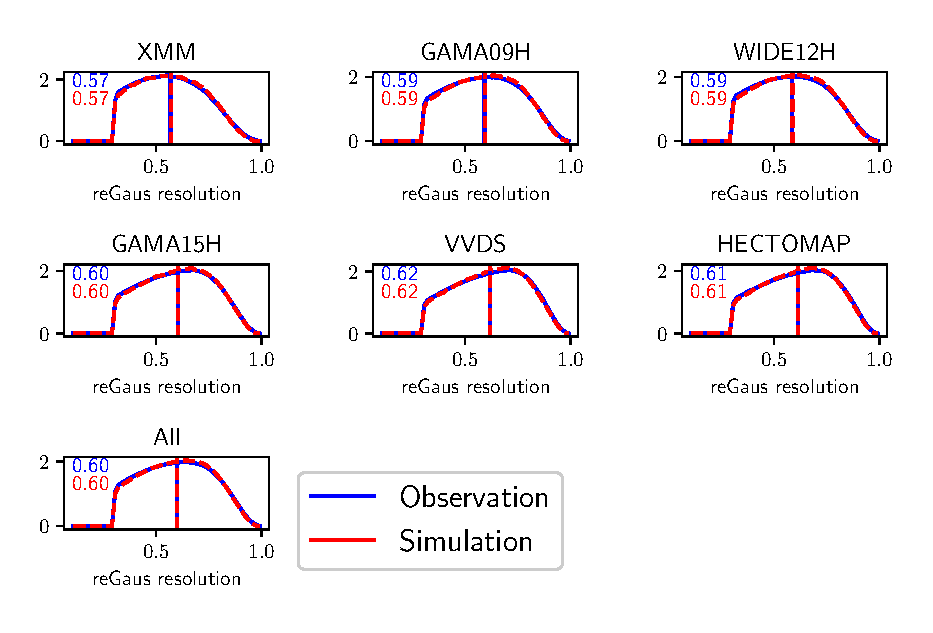
\includegraphics[width=0.9\textwidth]{resolutionDis_reCheck.eps}
}
\caption{The first 6 panels compare the number histograms of resolution between
    the observation and the simulation for galaxies in 6 fields of the second
    year HSC shape catalog. The last panel shows the histograms for the
    galaxies in all of the fields. The blue solid lines are for the observation
    and the red dashed lines are for the simulation.
    }
\end{figure*}


\begin{figure*}[ht!]
\centering{
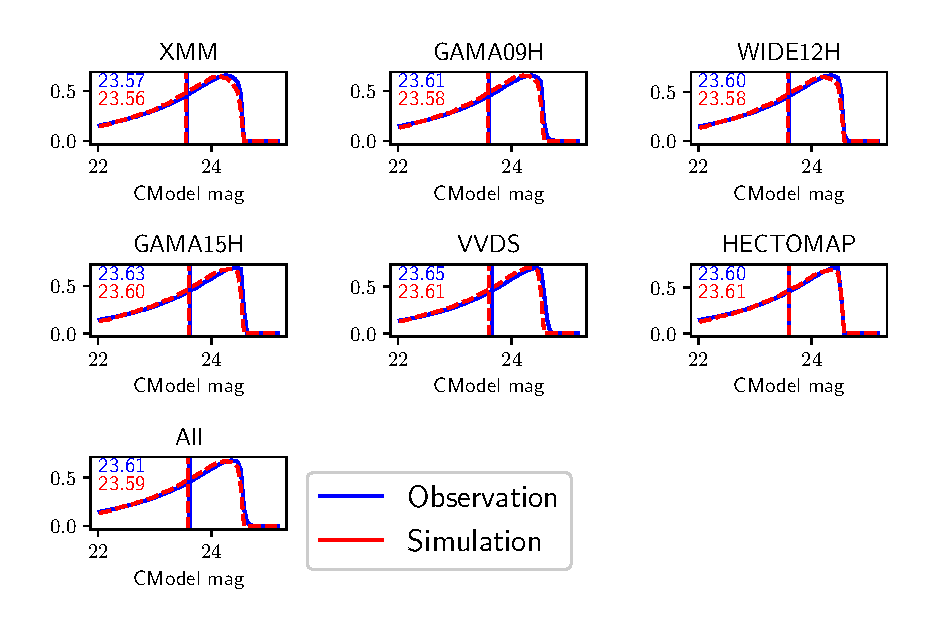
\includegraphics[width=0.9\textwidth]{magDis_reCheck.eps}
}
\caption{The first 6 panels compare the number histograms of CModel magnitude
    between the observation and the simulation for galaxies in 6 fields of the
    second year HSC shape catalog. The last panel shows the histograms for the
    galaxies in all of the fields. The blue solid lines are for the observation
    and the red dashed lines are for the simulation.
    }
\end{figure*}

\begin{figure*}[ht!]
\centering{
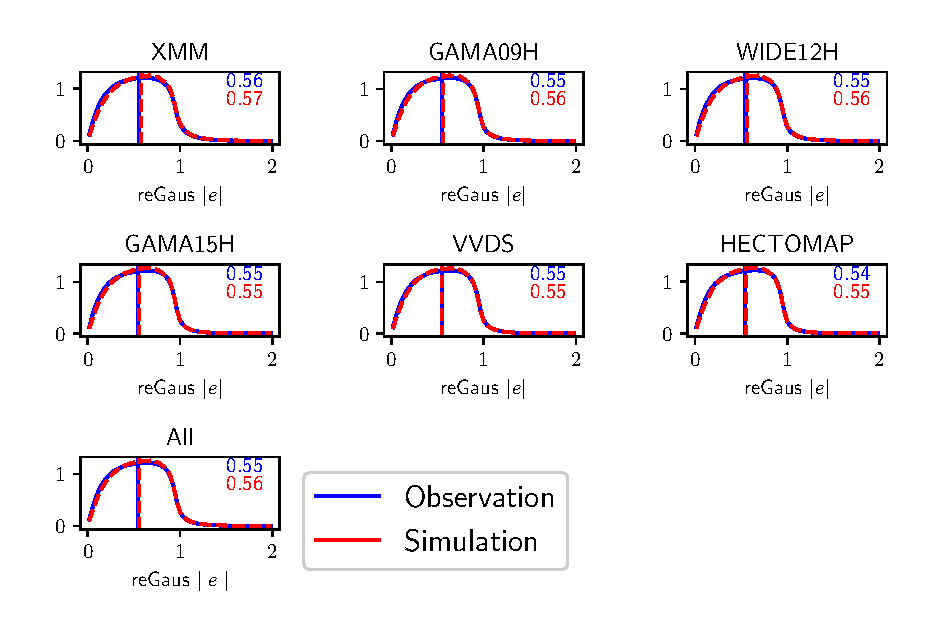
\includegraphics[width=0.9\textwidth]{absEDis_reCheck.eps}
}
\caption{The first 6 panels compare the number histograms of amplitude of
    ellipticity measured by re-gaussianization algorithm  between the
    observation and the simulation for galaxies in 6 fields of the second year
    HSC shape catalog. The last panel shows the histograms for the galaxies in
    all of the fields. The blue solid lines are for the observation and the red
    dashed lines are for the simulation.
    }
\end{figure*}


\begin{figure*}[ht!]
\centering{
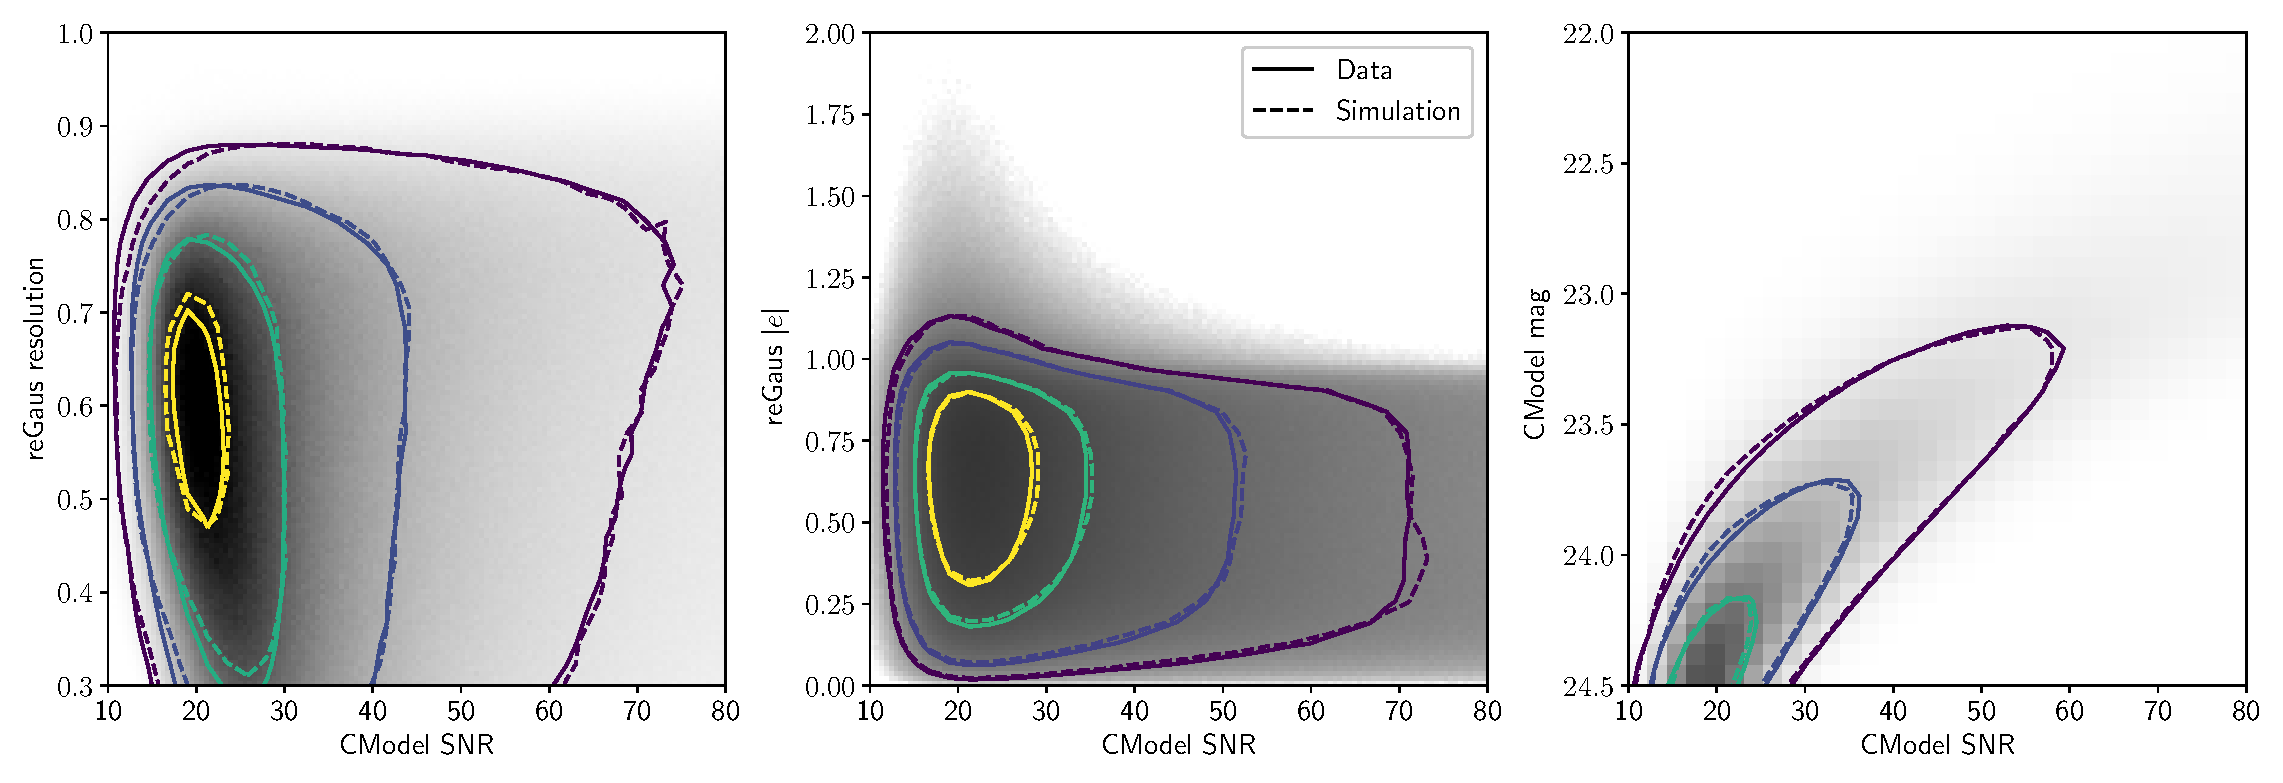
\includegraphics[width=0.9\textwidth]{galDis2D-final_reCheck.eps}
}
\caption{The $2$-D histograms of the simulation and the observation. The panels
    from left to right show the (SNR, resolution) histogram, (SNR, $\mid e
    \mid$) histogram and (SNR, CModel magnitude), respectively. The solid lines
    show the contours of the observation and the dashed lines show the contours
    of the simulation.
    }
\end{figure*}



\subsection{Optimization}
\label{subsec:optimal}
\begin{equation}
\sigma_e = 0.277 (\frac{\rm{SNR}}{20})^{-0.962} (\frac{\rm{res}}{0.5})^{-1.002}
\end{equation}


\begin{figure*}[ht!]
\centering{
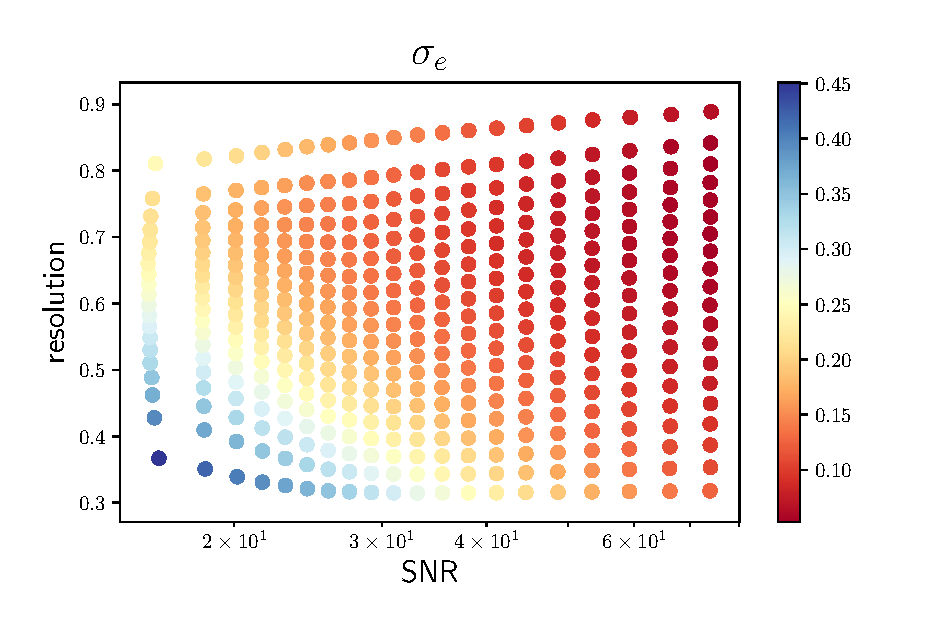
\includegraphics[width=0.45\textwidth]{sigmae_estimated.eps}
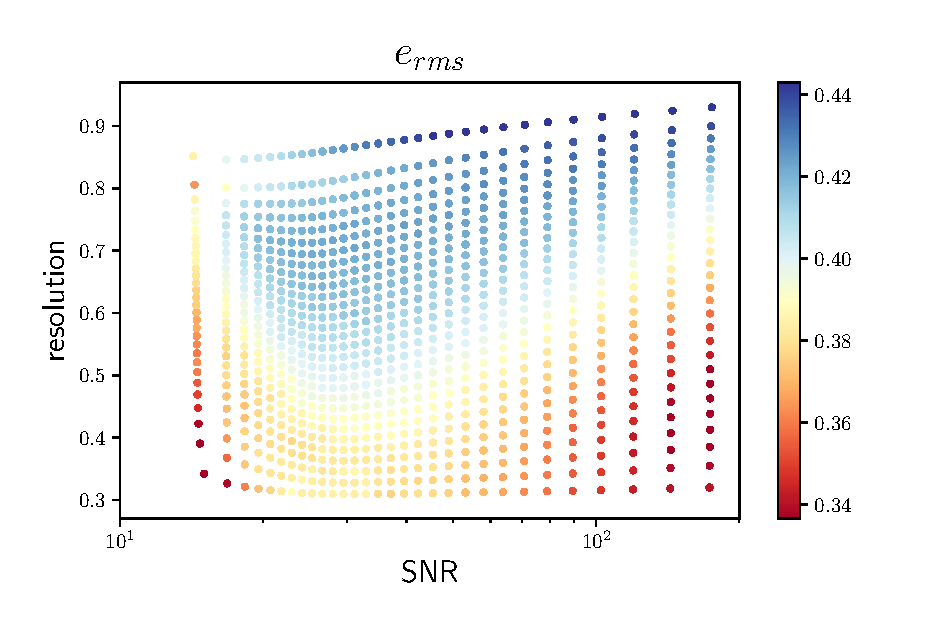
\includegraphics[width=0.45\textwidth]{intrinsicshape_2d.eps}
}
\caption{The left panel shows the shape measurement error per component
    ($\sigma_e$) estimated with the simulation in different (SNR, resolution)
    bins.  The right panel shows the intrinsic shape per component
    ($e_{\rm{RMS}}$) as function of (SNR, resolution).
    }
\end{figure*}

\subsection{Calibration}

\subsubsection{Shear Bias}

\begin{figure*}[ht!]
\centering{
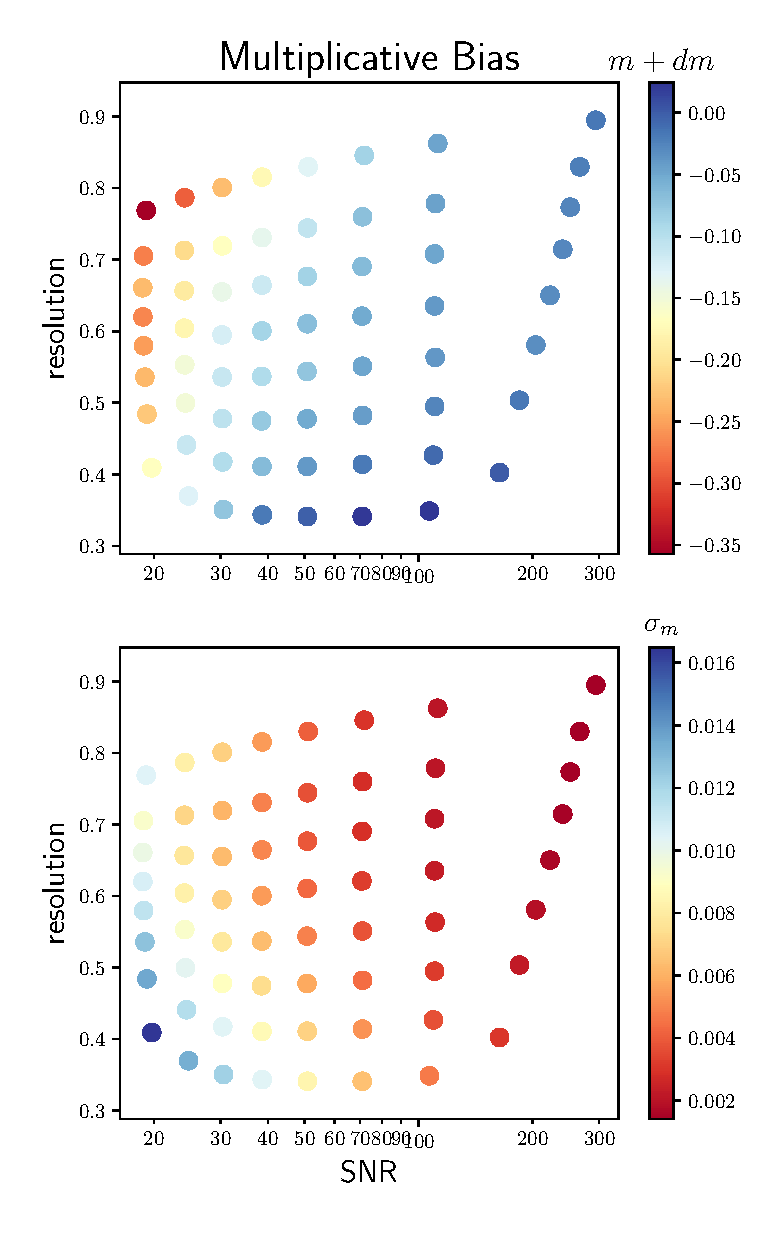
\includegraphics[width=0.45\textwidth]{shear_m_2d.eps}
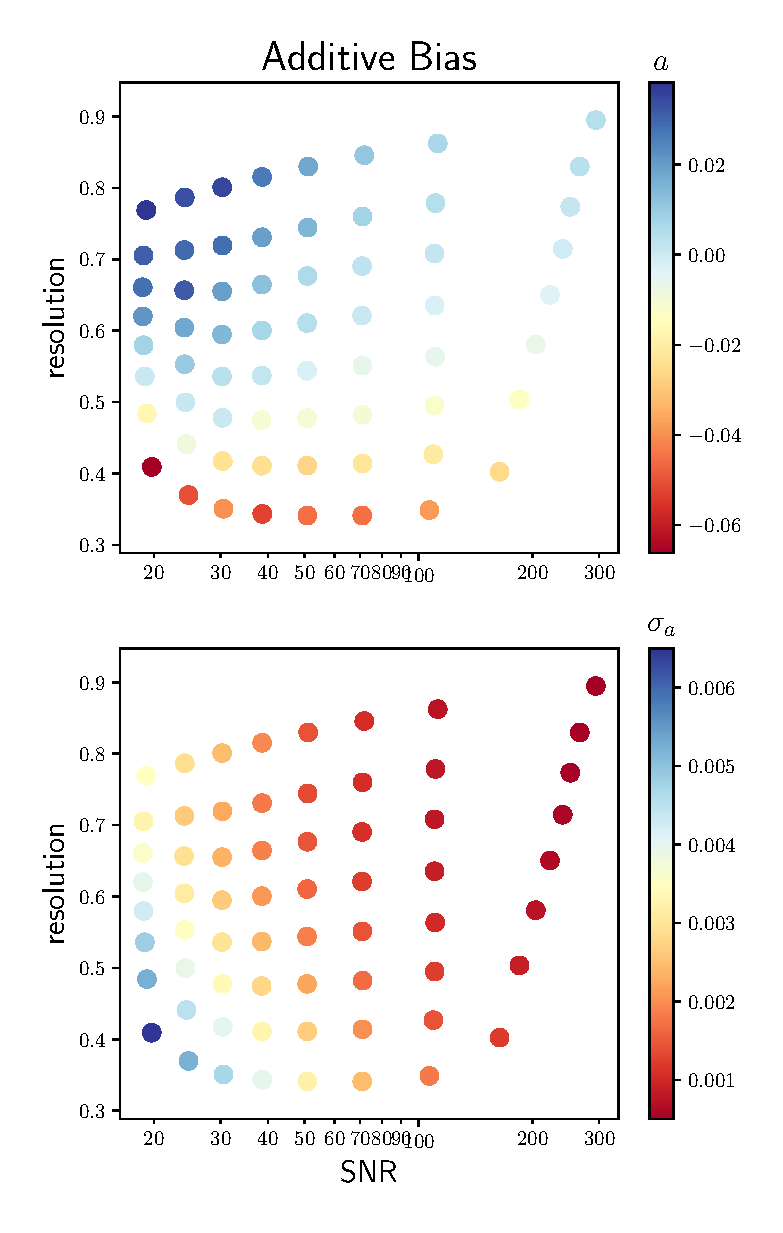
\includegraphics[width=0.45\textwidth]{shear_a_2d.eps}
}
\caption{The left panels show the multiplicative bias and the standard
    deviation of the multiplicative bias estimated in (SNR,resolution) bins
    with the simulation.  The right panels show the additive bias and the
    standard deviation of the additive bias estimated in (SNR,resolution) bins
    with the simulation.
    }
\end{figure*}

\begin{equation}
\hat{g}_{(1,2)}=\frac{\sum_i w_i e_{(1,2),i} }{2\res (1+\hat{m}) \sum_i w_i}-\frac{\hat{c}_{(1,2)}}{1+\hat{m}}
\end{equation}


\begin{equation}
m + \rm{const.} \propto (\frac{\rm{res}}{0.5})^{1.66}(\frac{\rm{snr}}{20})^{-1.24}
\end{equation}
\begin{equation}
a \propto (\rm{res}-0.61)(\frac{\rm{snr}}{20})^{-0.94}
\end{equation}

\subsubsection{Weight Bias}
\begin{figure*}[ht!]
\centering{
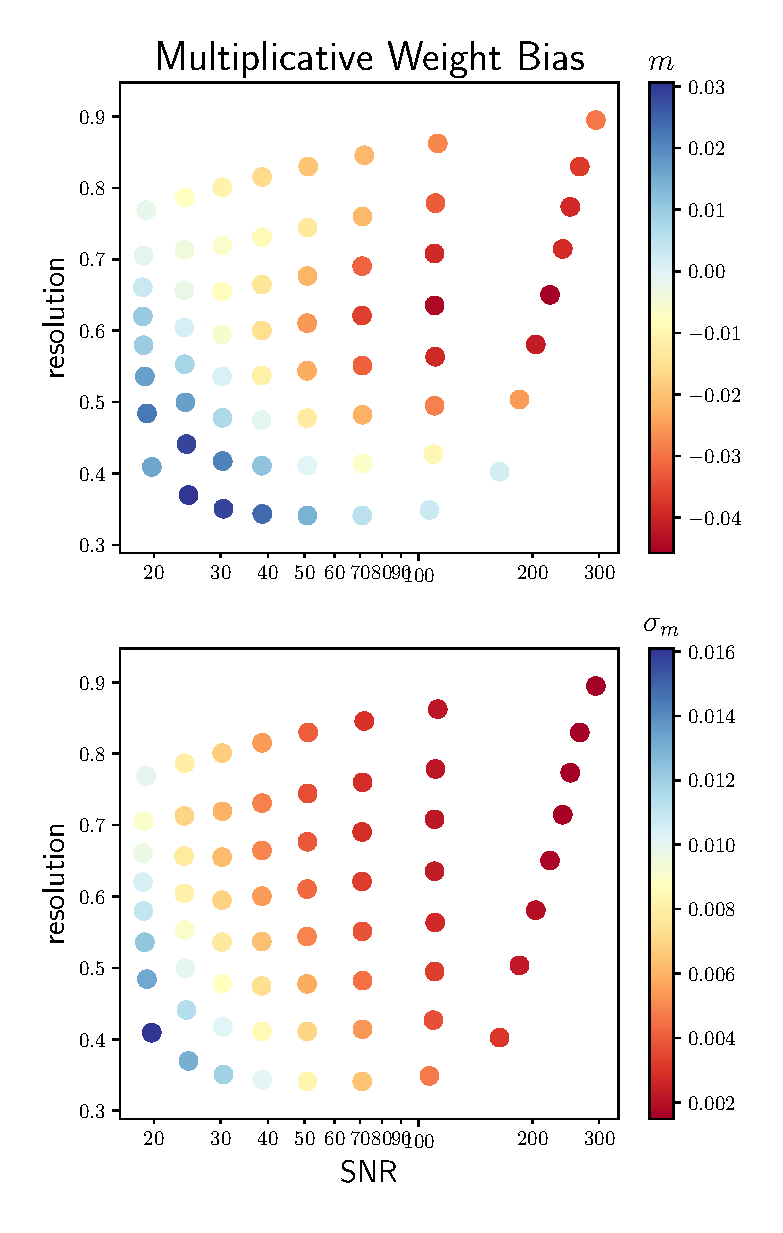
\includegraphics[width=0.45\textwidth]{weightBias_m_2d.eps}
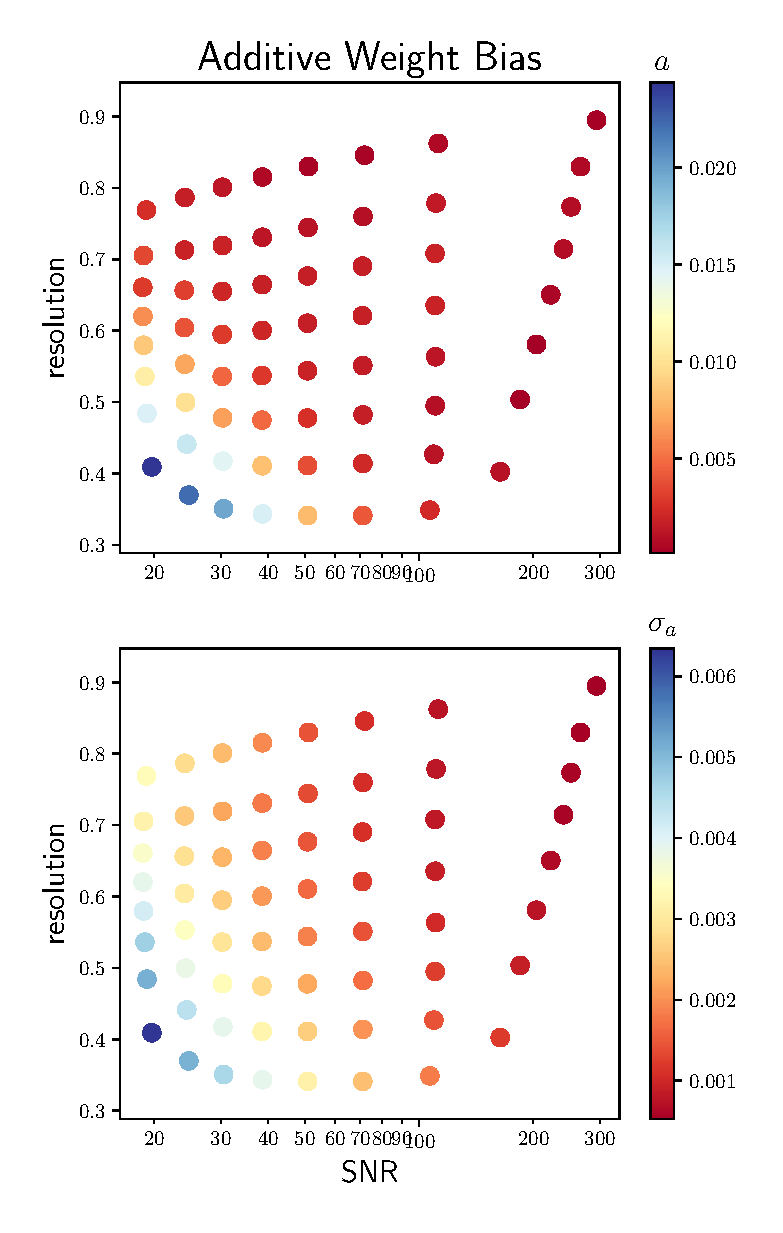
\includegraphics[width=0.45\textwidth]{weightBias_a_2d.eps}
}
\caption{The left panels show the multiplicative weight bias and the standard
    deviation of the multiplicative bias estimated in (SNR,resolution) bins
    with the simulation.  The right panels show the additive weight bias and
    the standard deviation of the additive bias estimated in (SNR,resolution)
    bins with the simulation.
    }
\end{figure*}

\subsubsection{Redshift Dependence}
\begin{figure*}[ht!]
\centering{
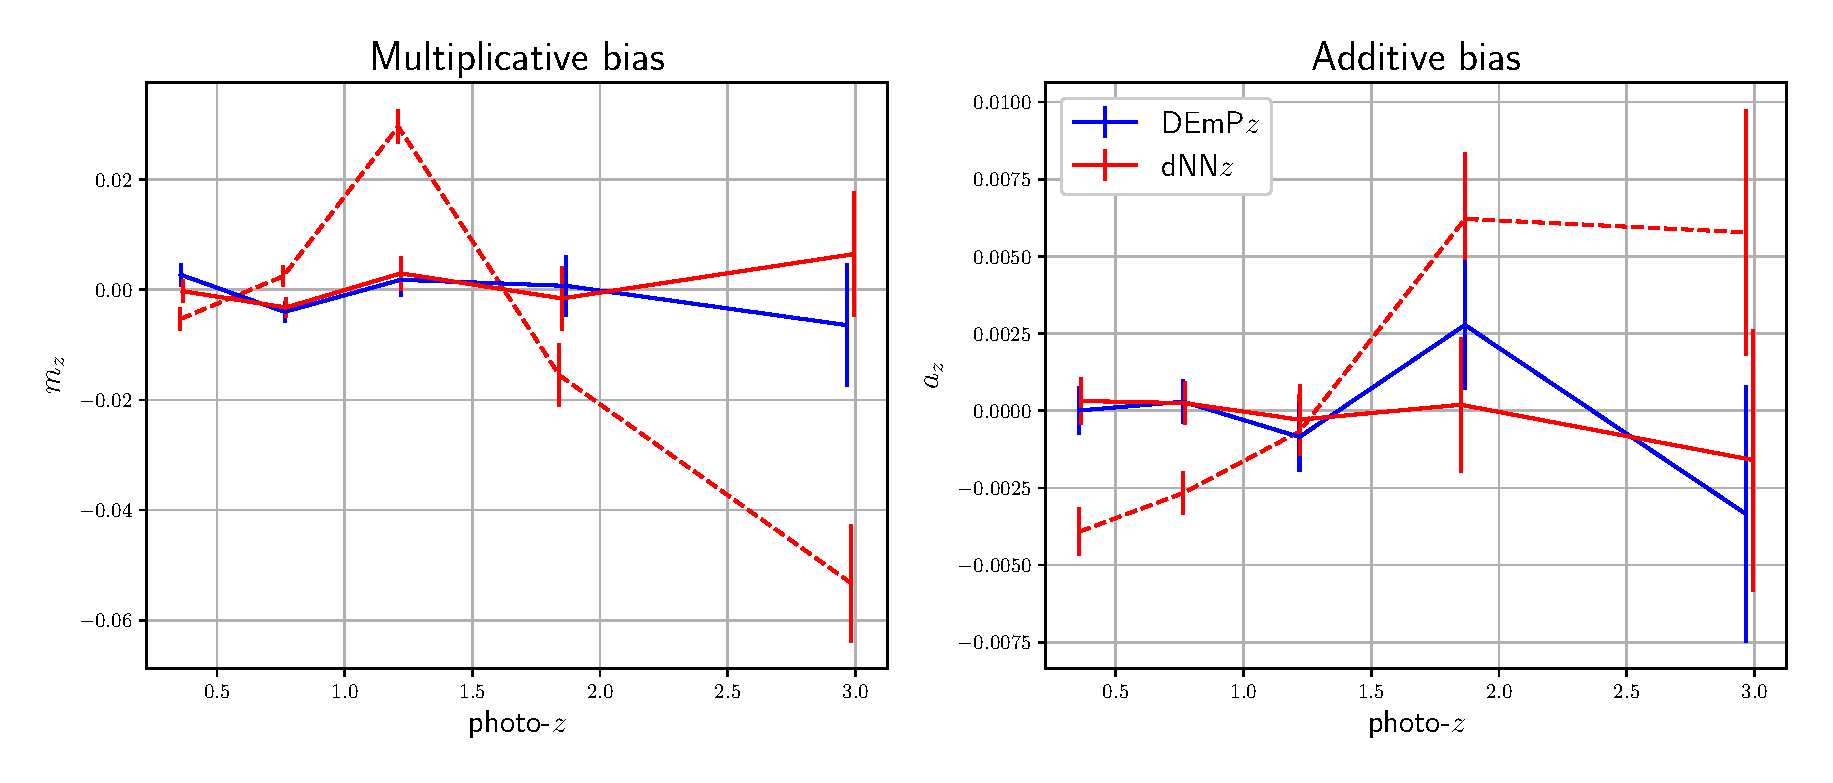
\includegraphics[width=0.9\textwidth]{calibration_residual_redshfits.eps}
}
\caption{The left panel shows the multiplicative bias residual estimated in
    photo-$z$ bins.  The right panel shows the additive bias residual estimated
    in photo-$z$ bins.  The red lines are for DEmPz, and the blue lines are for
    dNNz.  The dashed lines are the results before calibrating the redshift
    dependent bias, whereas the solid lines are the results after calibrating
    the redshift dependent bias using dNNz.
    }
\end{figure*}

\subsection{Sanity Test}
\subsubsection{Modeled Observables}
\begin{figure*}[ht!]
\centering{
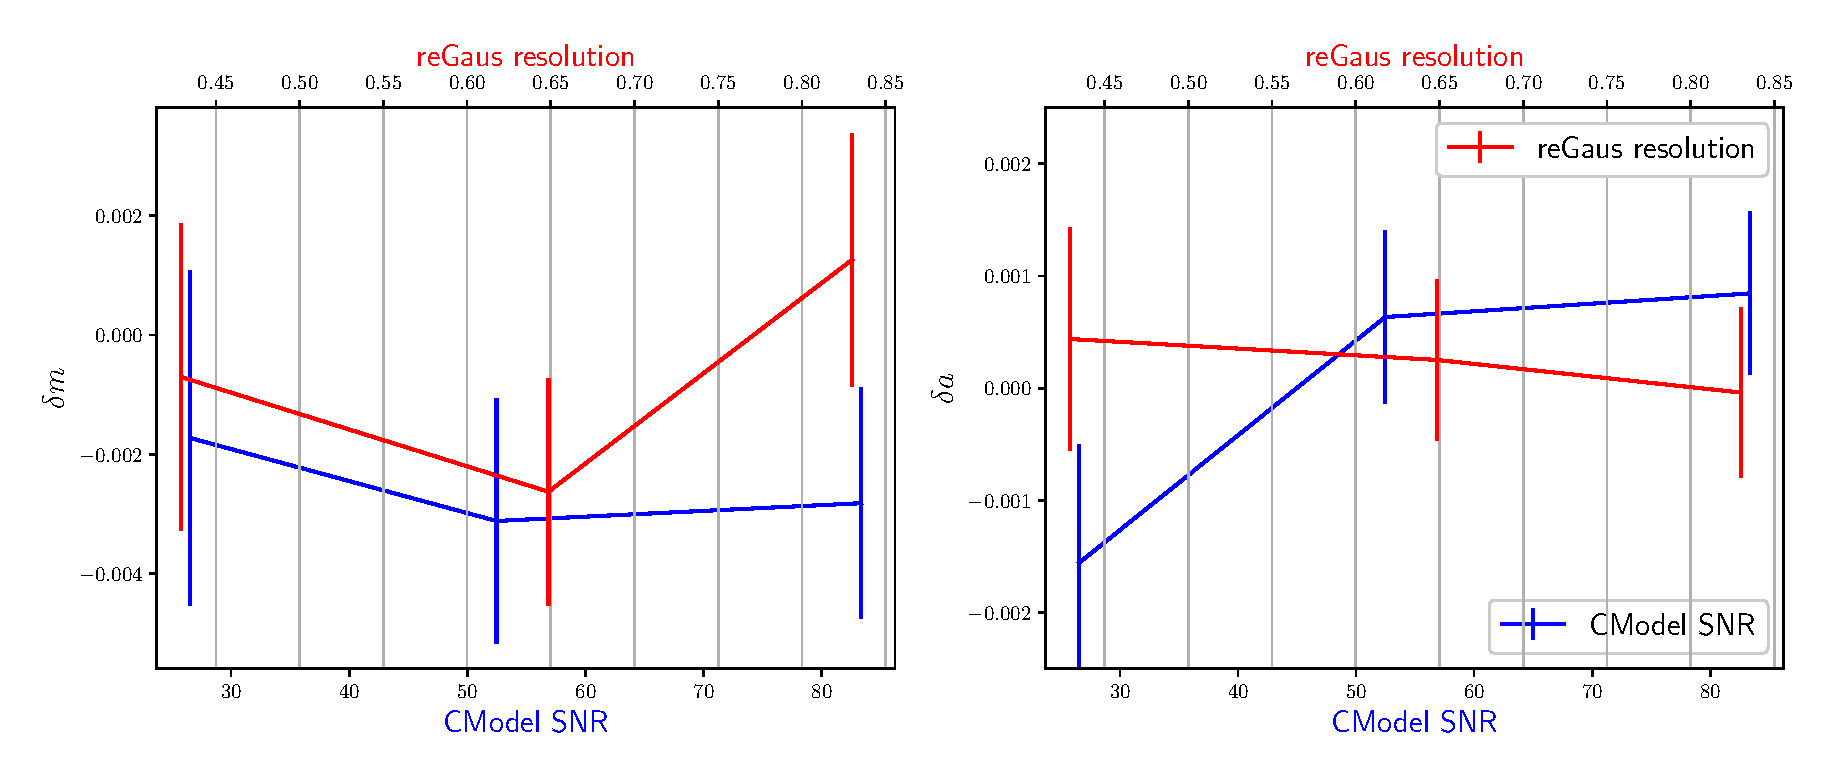
\includegraphics[width=0.9\textwidth]{calibration_residual_modeled.eps}
}
\caption{The dependence of calibration residuals the modeled properties.
        }
\end{figure*}

\subsubsection{Marginalized Observables}
\begin{figure*}[ht!]
\centering{
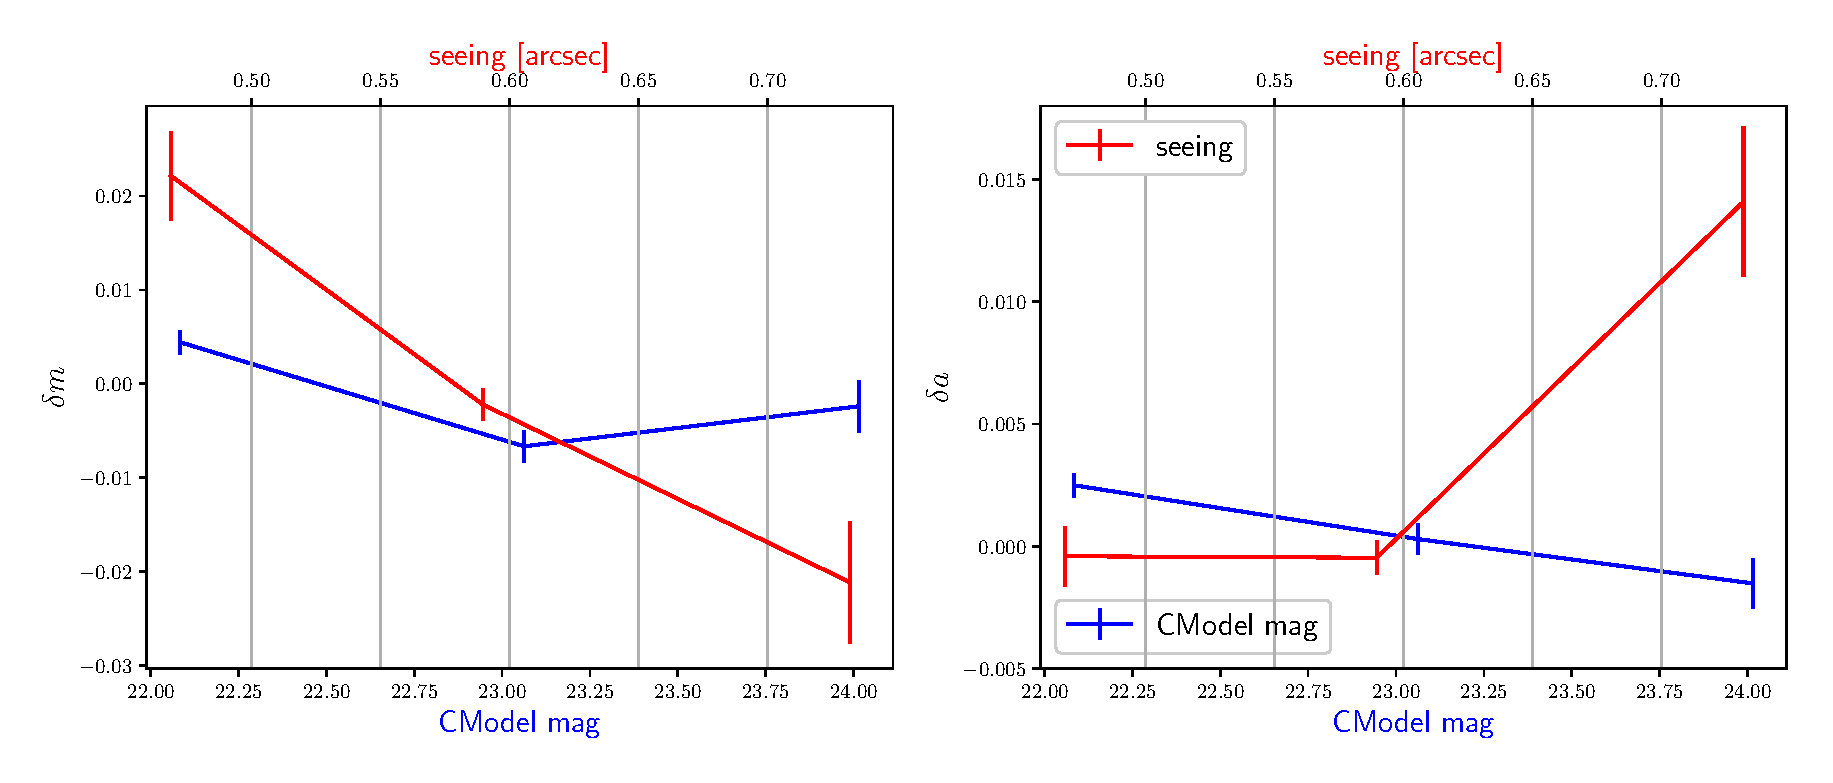
\includegraphics[width=0.9\textwidth]{calibration_residual_marginalized.eps}
}
\caption{The dependence of calibration residuals the marginalized properties.
        }
\end{figure*}

\subsection{Selection Bias}

\begin{figure*}[ht!]
\centering{
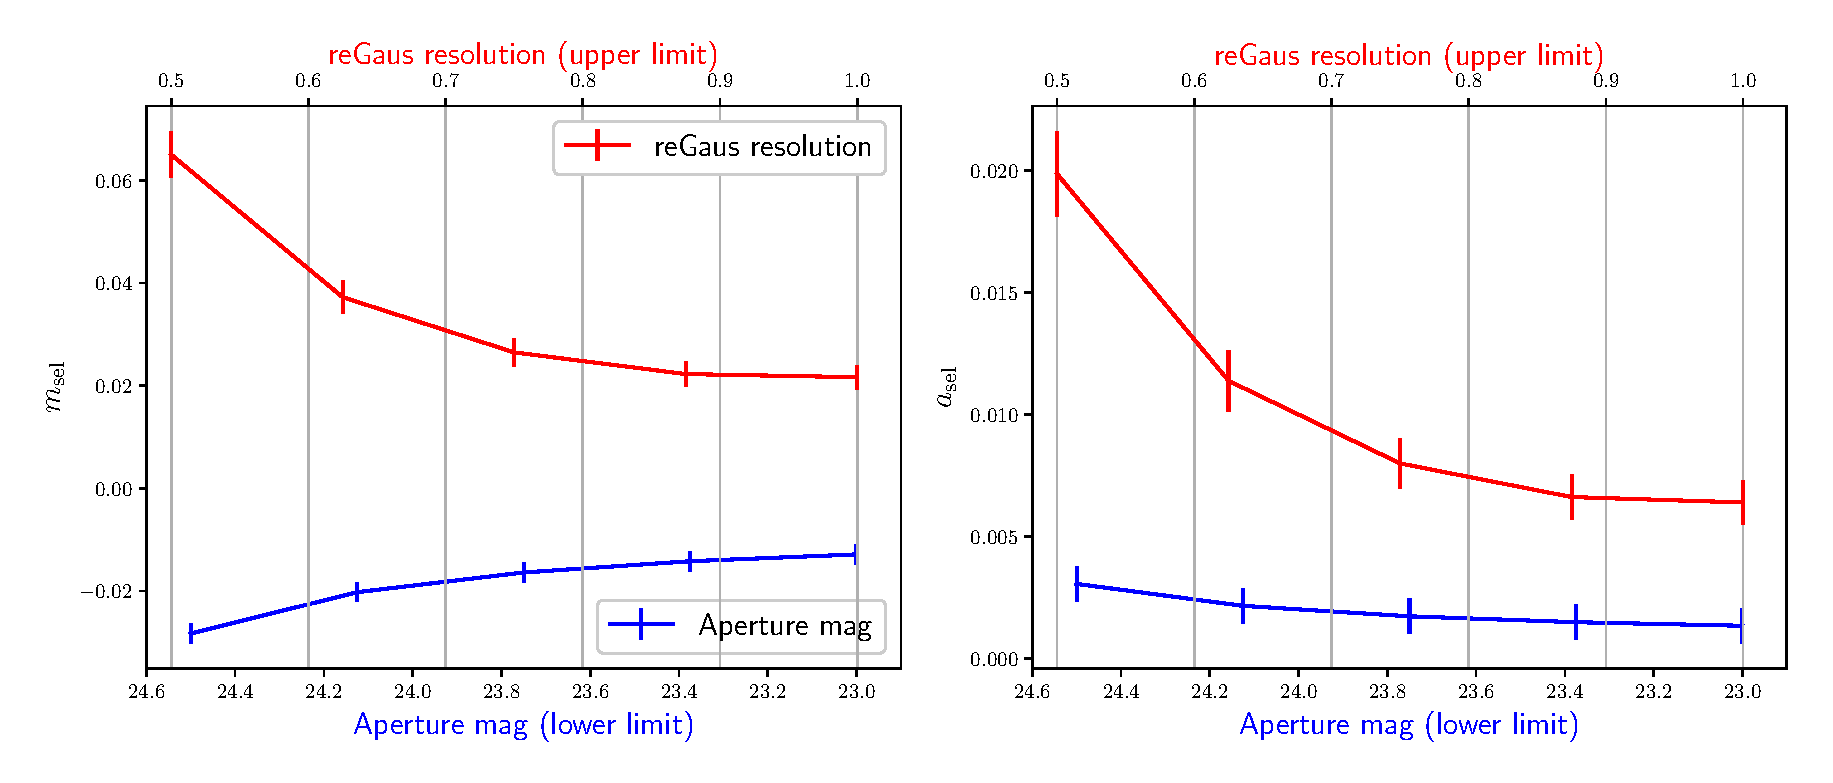
\includegraphics[width=0.9\textwidth]{selBias_res_magA10.eps}
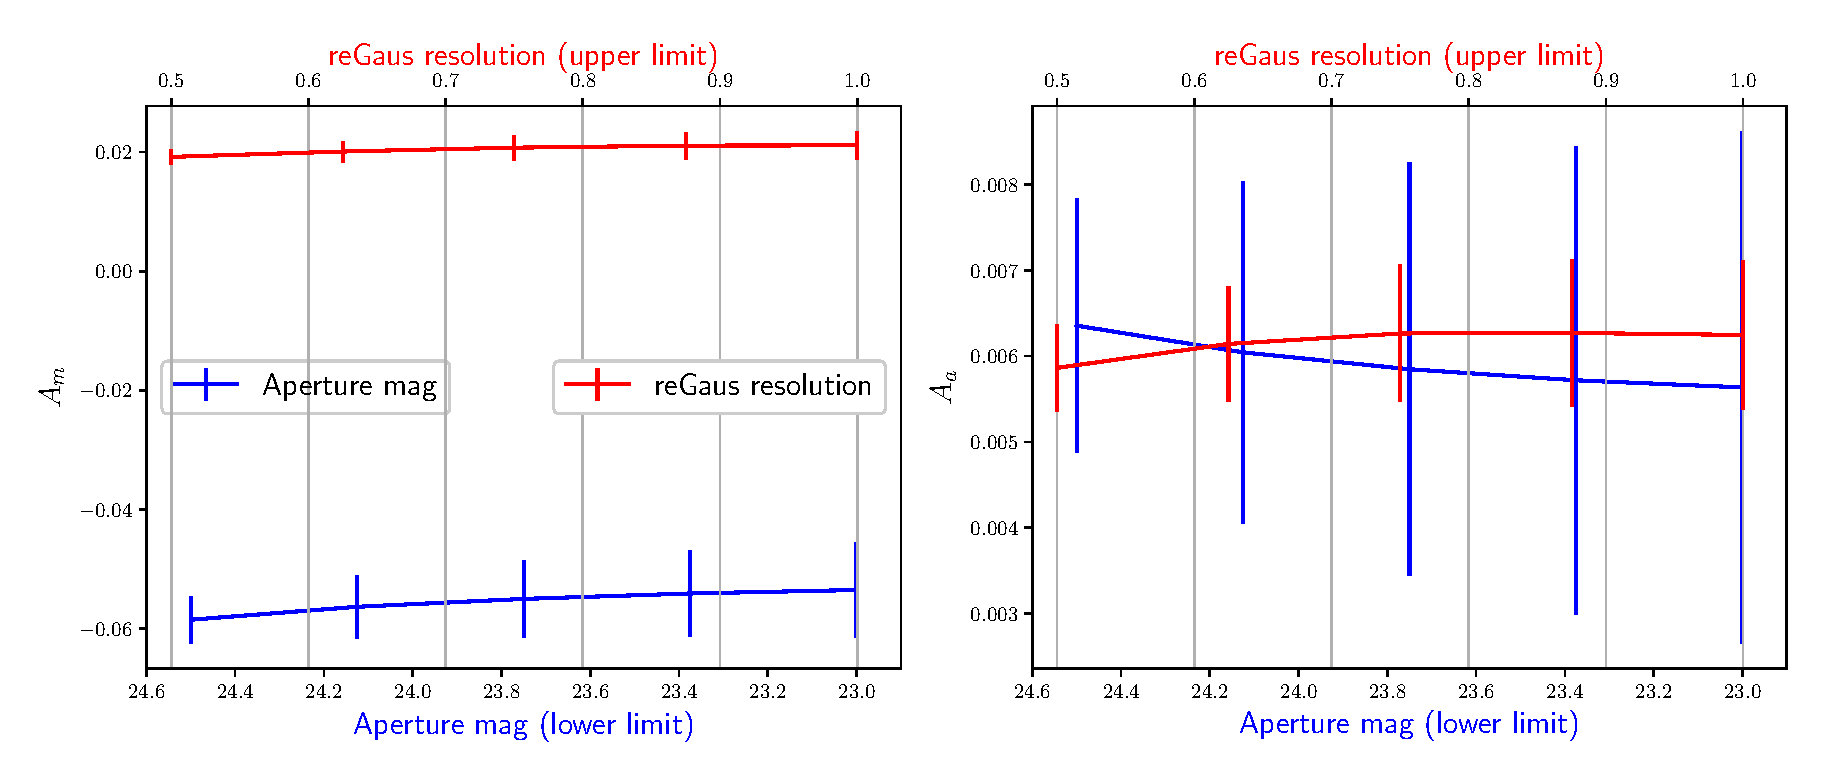
\includegraphics[width=0.9\textwidth]{selBias_ratio_res_magA10.eps}
}
\caption{
        }
\end{figure*}

\begin{table*}
\centering
  \begin{tabular}{ll} \hline
    Output properties & Meaning \\ \hline
\multicolumn{2}{c}{Optimization} \\ \hline
\texttt{i$\_$hsmshaperegauss$\_$derived$\_$sigma$\_$e}& Error due to photon noise \\ \hline
\texttt{i$\_$hsmshaperegauss$\_$derived$\_$rms$\_$e}  & Shape noise\\ \hline
\texttt{i$\_$hsmshaperegauss$\_$derived$\_$weight}    & weak lensing shape weight\\ \hline
\multicolumn{2}{c}{Calibration} \\ \hline
\texttt{i$\_$hsmshaperegauss$\_$derived$\_$shear$\_$bias$\_$m} & multiplicative bias\\ \hline
\texttt{i$\_$hsmshaperegauss$\_$derived$\_$shear$\_$bias$\_$c1}& the first component of additive bias\\ \hline
\texttt{i$\_$hsmshaperegauss$\_$derived$\_$shear$\_$bias$\_$c2}& the second component of additive bias\\ \hline
\hline
  \end{tabular}
  \caption{}
\end{table*}

\subsection{Characterization}
\begin{figure*}[ht!]
\centering{
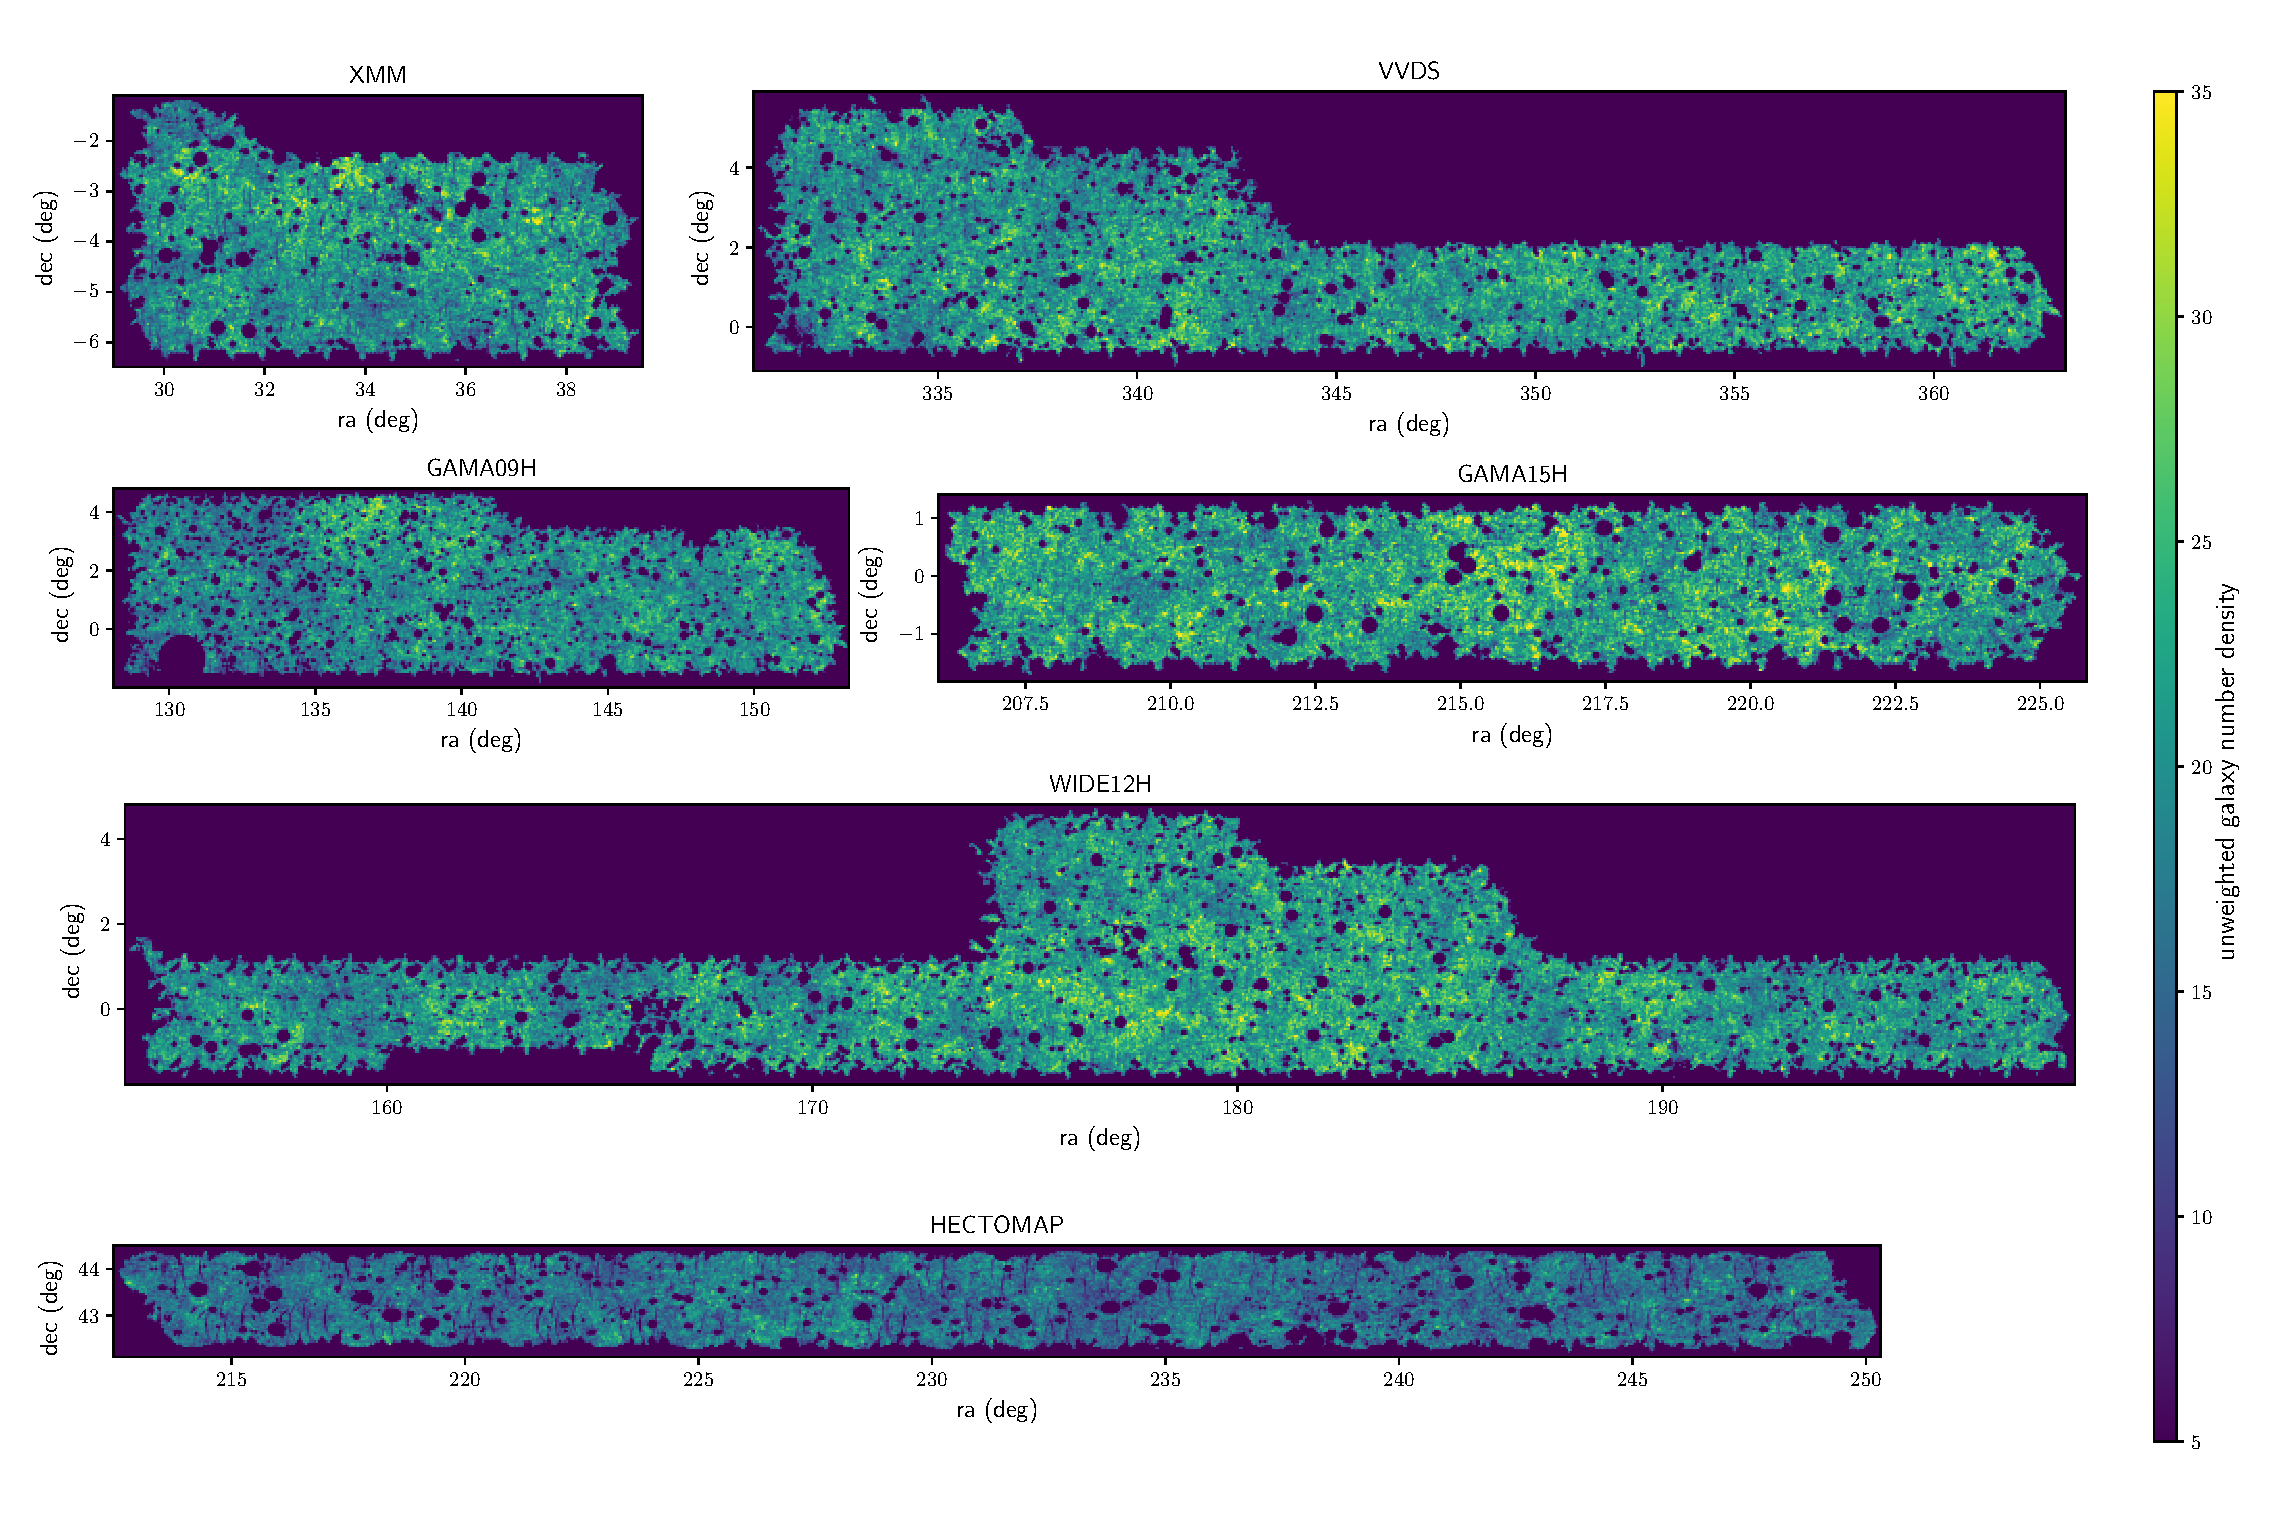
\includegraphics[width=0.9\textwidth]{densityMap.eps}
}
\caption{The unweighted galaxy number density map of the second year HSC shape
    catalog. The pixel scale is one arcmin.
    }
\end{figure*}

\begin{figure*}[ht!]
\centering{
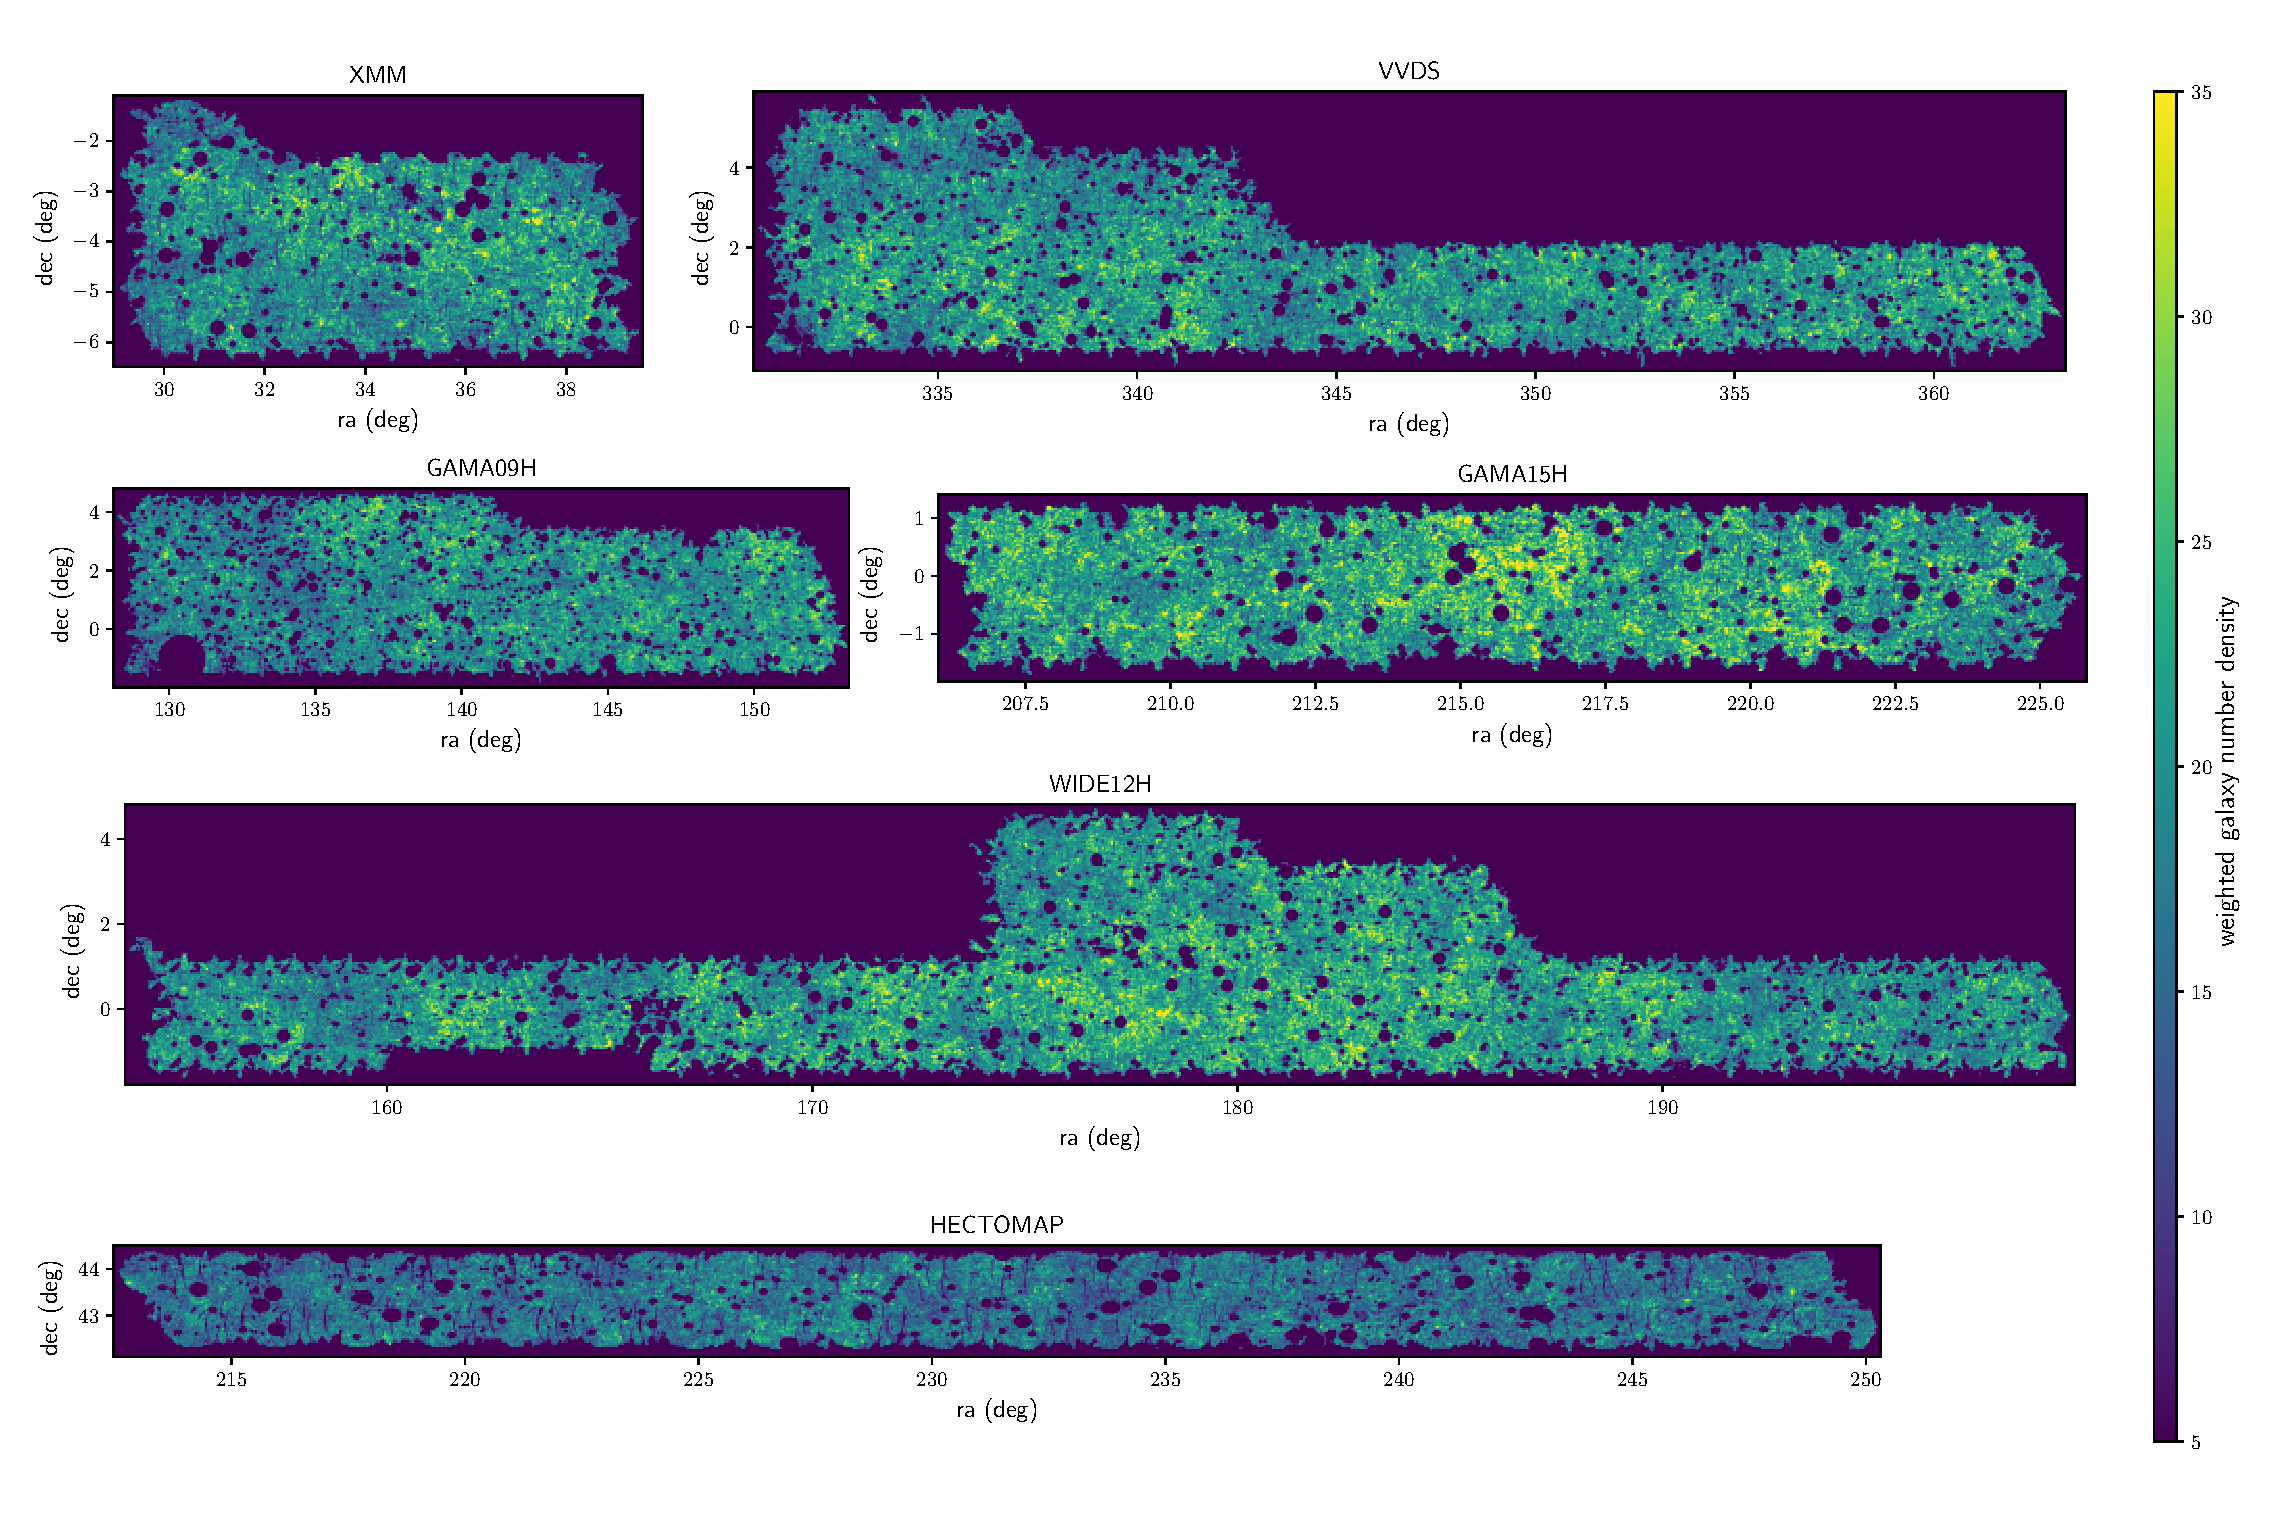
\includegraphics[width=0.9\textwidth]{wsMap.eps}
}

\caption{The weighted galaxy number density map of the second year HSC shape
    catalog. The pixel scale is one arcmin.
    }
\end{figure*}

\begin{enumerate}
    \item star contamination
    \item seeing density relation
\end{enumerate}
